\documentclass{article}
\usepackage[utf8]{inputenc}
\usepackage{graphicx}
\usepackage[left=3cm, right=4cm, top=2cm]{geometry}

\title{Práctica Simbólica -  SI}
\author{David Rodríguez Bacelar y Juan Ramón Pérez García}
\date{\today}

\begin{document}

\maketitle

\section{Ejercicio 1. Búsqueda Informada}

\bigskip\bigskip

\subsection{Búsqueda Avara}

\bigskip

\resizebox{\textwidth}{!} {
    \begin{tabular}{l|l|l}
        \hline
        \textit{Paso} & \textit{Frontera}                  & \textit{Explorados}             \\ \hline
        1             & start(2)                         & -                               \\ \hline
        2             & A(6), B(4), C(6)            & start(0)                        \\ \hline
        3             & A(6), C(6), E(2)            & start(0), B(10)                 \\ \hline
        4             & A(6), C(6), D(2), end(0) & start(0), B(10), E(12)          \\ \hline
        5             & A(6), C(6), D(2)            & start(0), B(10), E(12), end(18) \\ \hline
    \end{tabular}
}

\bigskip\bigskip
\subsection{Búsqueda A*}

\bigskip

\resizebox{\textwidth}{!} {
    \begin{tabular}{c|l|l}
    \hline
    \textit{Paso} & \textit{Frontera}          & \textit{Explorados}                              \\ \hline
    1    & start(0+2)                          & -                                                \\ \hline
    2    & A(5+6), B(10+4), C(5+6)             & start(0)                                         \\ \hline
    3    & E(9+2), B(10+4), C(5+6)             & start(0), A(5)                                   \\ \hline
    4    & E(9+2), B(9+4), F(11+3)             & start(0), A(5), C(5)                             \\ \hline
    5    & D(13+2), end(15+0), B(9+4), F(11+3) & start(0), A(5), C(5), E(9)                       \\ \hline
    6    & D(13+2), end(15+0), F(11+3)         & start(0), A(5), C(5), E(9), B(9)                 \\ \hline
    7    & D(13+2), end(14+0)                  & start(0), A(5), C(5), E(9), B(9), F(11)          \\ \hline
    8    & D(13+2)                             & start(0), A(5), C(5), E(9), B(9), F(11), end(14) \\ \hline
    \end{tabular}
}

\bigskip\bigskip
\subsection{Resultados:}
A pesar de que la Búsqueda Avara encuentra la solución expandiendo muchos menos nodos que A*, ésta no es óptima. En cambio,
A* utiliza una estrategia de búsqueda que, si se apoya en una heurística consistente, logra encotrar el camino óptimo (aunque como
vemos también, sacrificando algo más de complejidad temporal y espacial).
\newpage
\section{Ejercicio 2. Búsqueda con Graph Search}
\begin{enumerate}
    \setlength\itemsep{2em}
    \item 
        Distancias:
        
        \bigskip
        \begin{tabular}{l|l|l|l|l|l}
            \hline
                            & \textit{Inicio} & \textit{Uno} & \textit{Dos} & \textit{Tres} & \textit{Meta} \\ \hline
            \textit{Inicio} & 0               & 8            & 6            & 8             & 10            \\ \hline
            \textit{Uno}    & 8               & 0            & 6            & 8             & 10            \\ \hline
            \textit{Dos}    & 6               & 6            & 0            & 4             & 6             \\ \hline
            \textit{Tres}   & 8               & 8            & 4            & 0             & 2             \\ \hline
            \textit{Meta}   & 10              & 10           & 6            & 2             & 0             \\ \hline
        \end{tabular}
        
    \item
        Estados:
        \begin{itemize}
            \item[$-$]  Robot en 'Inicio'. \{inicio\}
            \item[$-$]  Robot en 'Uno' con paquete 1. \{Uno(1)\}
            \item[$-$]  Robot en 'Dos' con paquete 2. \{Dos(2)\}
            \item[$-$]  Robot en 'Tres' con paquete 3. \{Tres(3)\}
            \item[$-$]  Robot en 'Tres' con paquetes 1 y 3. \{Tres(1,3)\}
            \item[$-$]  Robot en 'Dos' con paquetes 1 y 2. \{Dos(1,2)\} 
            \item[$-$]  Robot en 'Uno' con paquetes 2 y 1. \{Uno(2,1)\}
            \item[$-$]  Robot en 'Tres' con paquetes 2 y 3. \{Tres(2,3)\}
            \item[$-$]  Robot en 'Uno' con paquetes 3 y 1. \{Uno(3,1)\}
            \item[$-$]  Robot en 'Dos' con paquetes 3 y 2. \{Dos(3,2)\}
            \item[$-$]  Robot en 'Tres' con paquetes 1, 2 y 3. \{Tres(1,2,3)\}
            \item[$-$]  Robot en 'Dos' con paquetes 1, 2 y 3. \{Dos(1,2,3)\}
            \item[$-$]  Robot en 'Uno' con paquetes 1, 2 y 3. \{Uno(1,2,3)\}
            \item[$-$]  Robot en 'Meta'. \{meta\}
        \end{itemize}
        
    \item
        Acciones:
        \begin{itemize}
            \setlength\itemsep{1em}
            \item[$\diamond$] Ir a 'Uno' y coger el paquete. \\\textit{PreCD}: No se han recogido todos los paquetes y tampoco el de la localidad 'Uno'.
            \item[$\diamond$] Ir a 'Uno' y coger el paquete. \\\textit{PreCD}: No se han recogido todos los paquetes y tampoco el de la localidad 'Dos'.
            \item[$\diamond$] Ir a 'Tres' y coger el paquete. \\\textit{PreCD}: No se han recogido todos los paquetes y tampoco el de la localidad 'Tres'.
            \item[$\diamond$] Ir a 'Meta'. \\\textit{PreCD}: Todos los paquetes han sido recogidos.
        \end{itemize}
    
    \newpage
    \item
        Heurística: \bigskip\\
        La heurística utilizada será la distanicia mínima a la meta desde cualquier localidad, sumado al coste de levantar los paquetes restantes. 
        Es una buena heurística ya que siempre nos proporciona costes de camino subestimados 'relajando' el problema; para que el coste del camino real
        fuese igual al estimado, sería necesario que los paquetes restantes se encontraran en el camino de distancia mínima hasta la meta (el mejor caso), por
        lo que en otro escenario distinto a ese, el coste sería superior al estimado.
        \begin{equation}
            h(x)= d(x,meta) + Coste\_de\_levantar\_los\_paquetes\_restantes
        \end{equation}

    \item
        Grafo:
        \begin{figure}[h!]
            \centering
            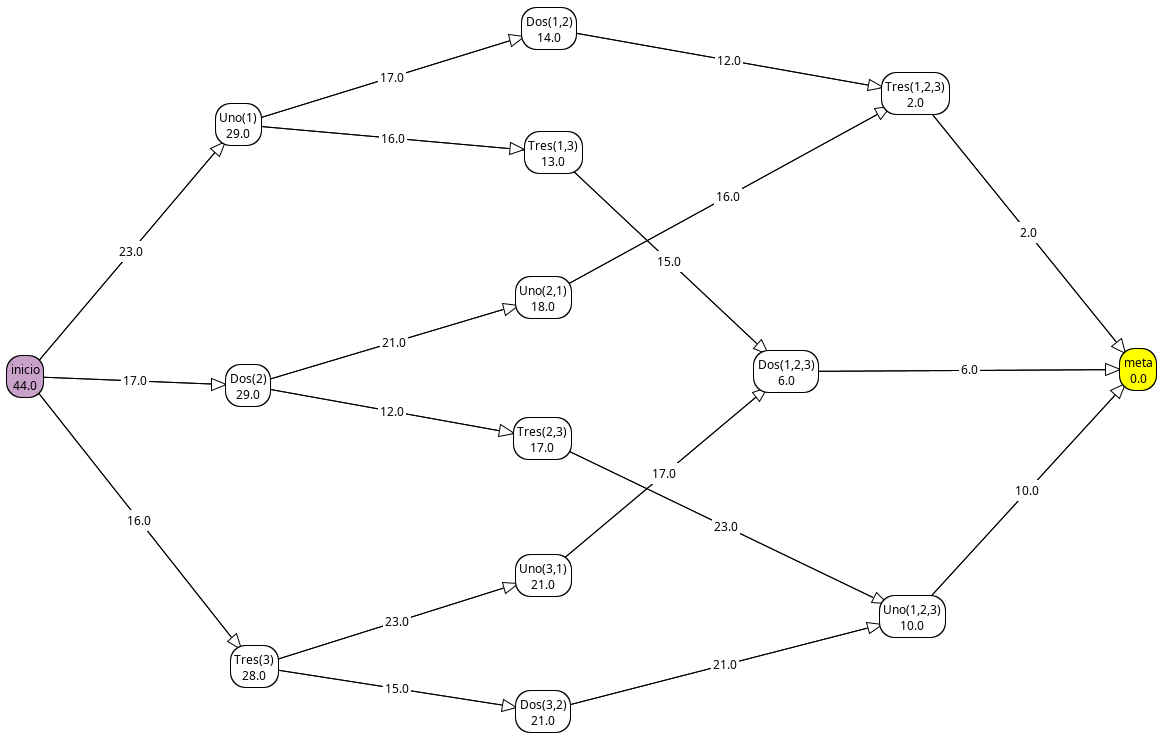
\includegraphics[height=200px]{graph.png}
            \label{fig:diagram1}
        \end{figure}

    \item
        Resultados:

        \begin{itemize}
            \item \underline{Depth First}:
                \begin{itemize}
                    \item Camino encontrado: inicio $\rightarrow$ Dos(2) $\rightarrow$ Tres(2,3) $\rightarrow$ Uno(1,2,3) $\rightarrow$ meta
                    \item Coste del camino: 62
                    \item Nodos expandidos: 5
                \end{itemize}
            \smallskip
            \item \underline{Breadth First}:
                \begin{itemize}
                    \item Camino encontrado: inicio $\rightarrow$ Dos(2) $\rightarrow$ Tres(2,3) $\rightarrow$ Uno(1,2,3) $\rightarrow$ meta
                    \item Coste del camino: 62
                    \item Nodos expandidos: 17
                \end{itemize}
            \smallskip
            \item \underline{Lowest Cost First}:
                \begin{itemize}
                    \item Camino encontrado: inicio $\rightarrow$ Uno(1) $\rightarrow$ Dos(1,2) $\rightarrow$ Tres(1,2,3) $\rightarrow$ meta
                    \item Coste del camino: 54
                    \item Nodos expandidos: 16
                \end{itemize}
            \smallskip
            \newpage
            \item \underline{Best First}:
                \begin{itemize}
                    \item Camino encontrado: inicio $\rightarrow$ Tres(3) $\rightarrow$ Dos(3,2) $\rightarrow$ Uno(1,2,3) $\rightarrow$ meta
                    \item Coste del camino: 62
                    \item Nodos expandidos: 5
                \end{itemize}
            \smallskip
            \item \underline{A*}:
                \begin{itemize}
                    \item Camino encontrado: inicio $\rightarrow$ Uno(1) $\rightarrow$ Dos(1,2) $\rightarrow$ Tres(1,2,3) $\rightarrow$ meta
                    \item Coste del camino: 54
                    \item Nodos expandidos: 10
                \end{itemize}           
        \end{itemize}
        \bigskip
        \textit{(Todas las busquedas han sido realizadas con selección de vecinos por orden alfabético)}

    \item
        Conclusiones y discusión:

        \setlength{\parindent}{2ex}
        El algoritmo que mejores resultados ofrece es \textit{A*} ya que, encontrando la solución óptima, expande menos nodos que \textit{Lowest Cost First}.
        \textit{A*} será, por lo general, el mejor algoritmo que garantize la optimalidad (y completitud) expandiendo el menor número de 
        nodos posibles en problemas no muy grandes, con factores de ramificación finitos y con la posibilidad de hallar una heurística consistente (como el nuestro).
        La ventaja que tienen los algoritmos como \textit{Best First} o o \textit{Depth First} es que hallan también una solución (aunque no óptima)
        expandiendo muy pocos nodos, ambos solo 5.

        Si variamos mínimamente el problema, los algoritmos como \textit{Breadth First} (que solo garantiza optimalidad cuando los costes de los caminos
        son constantes), \textit{Depth First} o \textit{Best First}, es muy probable que sigan sin encontrar soluciones óptimas; pero dado que los parámetros de nuestro problema
        son finitos (factor de ramificación, espacio de estados...) todos seguirían encontrando soluciones no óptimas. En el caso de \textit{Lowest Cost First} y
        \textit{A*}, las soluciones que encontrarían serían igualmente óptimas.
\end{enumerate}
\end{document}
